% mainly focus on problems of personalization in federated learning

\usepackage{nccmath}

\tikzset{%
  client/.style={
    rectangle,
    thick,
    draw,
    minimum size=0.7cm,
    text width=1cm,
    align=center
  },
  client missing/.style={
    draw=none, 
    scale=2,
    text height=0.333cm,
    execute at begin node=$\cdots$
  },
}
\usepackage{transparent}

\usepackage{listings}

\lstdefinestyle{mystyle}{
    backgroundcolor=\color{zkbackground},   
    commentstyle=\color{green},
    keywordstyle=\color{magenta},
    numberstyle=\tiny\color{gray},
    stringstyle=\color{purple},
    basicstyle=\ttfamily\footnotesize,
    breakatwhitespace=false,         
    breaklines=true,                 
    captionpos=b,                    
    keepspaces=true,                 
    numbers=left,                    
    numbersep=5pt,                  
    showspaces=false,                
    showstringspaces=false,
    showtabs=false,                  
    tabsize=4
}

\begin{document}

%----------------------------------------------------------------------------------------
%	TITLE PAGE
%----------------------------------------------------------------------------------------

\title[Personalization]{Problems of Personalization in Federated Learning}
\date{2021-07-29}
\author[WEN Hao]{WEN Hao}

% \institute[北京航空航天大学] % Your institution as it will appear on the bottom of every slide, may be shorthand to save space
% {
% 数学科学学院 \\ % Your institution for the title page
% \medskip
% \textit{wenh06@gmail.com} % Your email address
% 北京航空航天大学 \\
% 数学科学学院 \qquad 北京航空航天大学
% }

% \logo{\includegraphics[height=1.5cm]{logo}}
% \logoii{\includegraphics[height=1cm]{logo2}}

% \date{\footnotesize 2021年4月13日} % Date, can be changed to a custom date

\setlength{\belowdisplayskip}{5pt} \setlength{\belowdisplayshortskip}{5pt}
\setlength{\abovedisplayskip}{5pt} \setlength{\abovedisplayshortskip}{5pt}

%------------------------------------------------

\begin{frame}
\titlepage % Print the title page as the first slide
\end{frame}
%------------------------------------------------

\begin{frame}
% \frametitle{Overview} % Table of contents slide, comment this block out to remove it
\tableofcontents % Throughout your presentation, if you choose to use \section{} and \subsection{} commands, these will automatically be printed on this slide as an overview of your presentation
\end{frame}

%------------------------------------------------

%------------------------------------------------
%	PRESENTATION SLIDES
%------------------------------------------------


% PPT version (read only share link): https://www.kdocs.cn/l/cigmbsd3uAI4


%------------------------------------------------

\section[Introduction]{引言}

%------------------------------------------------
% Page 1

\begin{frame}
\frametitle{引言}

联邦学习(Federated Learning)来源于机器(深度)学习模型分布式(Distributed)训练的需求

\begin{figure}
    \centering
    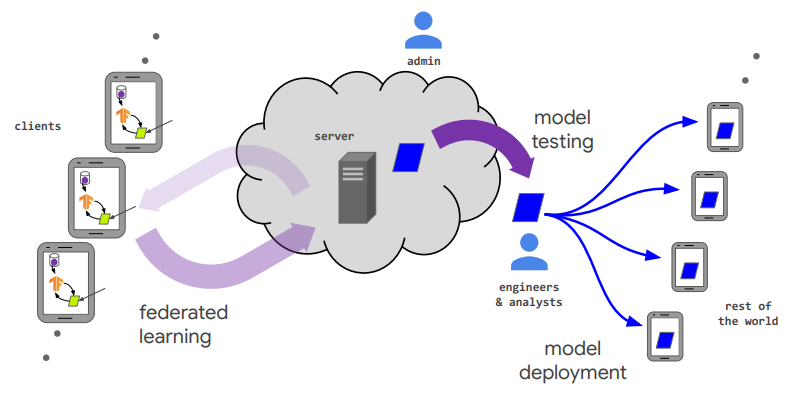
\includegraphics[width=\textwidth,keepaspectratio]{images/fl_overview.png}
\end{figure}

{\scriptsize
图片来源:\cite{kairouz2019advances_fl} Kairouz et al., Advances and open problems in federated learning, 2019
}

\end{frame}

%------------------------------------------------
% Page 15

\begin{frame}
\frametitle{引言}

这种分布式训练的需求多是当多个数据拥有方想要联合他们各自的数据训练机器学习模型,由于涉及隐私和数据安全等法律问题,或是数据庞大且过于分散导致的可行性问题,而不能将数据集中到一起进行模型训练而产生的。随着越来越严格的数据隐私方面的法律法规的施行,这种需求会越来越大。

\pause
\vspace{0.8em}

一般来说,在联邦学习的框架下,数据拥有方在不用给出己方数据的情况下,也可进行模型训练得到公共的模型$M_{fed}$,使得模型$M_{fed}$,与将数据集中到一起进行训练能得到的模型$M$,二者的预测值的偏差的期望能足够小。
$$\expectation_{z\sim\mathcal{D}} \lVert M_{fed}(z) - M(z) \rVert \leqslant \delta$$

\vspace{0.5em}

{\footnotesize 注:以下将数据拥有方统称为``节点''}

\end{frame}

%------------------------------------------------
% Page 15

\begin{frame}
\frametitle{联邦学习的定义}

综述文章\cite{kairouz2019advances_fl} Advances and open problems in federated learning (2019)给联邦学习下过如下的定义

\vspace{0.8em}

\begin{quote}
    ``Federated learning is a machine learning setting where multiple entities (clients) collaborate in solving a machine learning problem, under the coordination of a central server or service provider. Each client's raw data is stored locally and not exchanged or transferred; instead, focused updates intended for immediate aggregation are used to achieve the learning objective.''
\end{quote}

\end{frame}

%------------------------------------------------
% Page 15

\begin{frame}
\frametitle{联邦学习研究的一些核心的问题}

\begin{itemize}
    \item {\Large\bfseries EE (Efficiency \& Effectiveness)}
    \begin{itemize}
        \item[$\bullet$] {\large\bfseries Optimization}
        \vspace{0.5em}
        \item[$\bullet$] Compression
        \pause
        {\pgfsetfillopacity{0.4} \footnotesize
        }
    \end{itemize}
    \vspace{0.6em}
    {\pgfsetfillopacity{0.4} \footnotesize
    \item Privacy \& Security
    \begin{itemize}
        \item[$\bullet$] Differential Privacy (DP)
        \item[$\bullet$] Secure Multi-Party Computing (SMPC)
        \item[$\bullet$] Trusted Execution Environment (TEE)
        \item[$\bullet$] Homomorphic Encryption (HE)
    \end{itemize}
    \item Applications
    \begin{itemize}
        \item[$\bullet$] Medical
        \item[$\bullet$] Recommendation
        \item[$\bullet$] Finance
    \end{itemize}
    \item etc.
    }
\end{itemize}

\end{frame}

%------------------------------------------------

\section[Optim in FL]{联邦学习中的优化问题与算法}

%------------------------------------------------
% Page 15

\begin{frame}
\frametitle{问题描述}

一般来说,联邦学习中我们考虑的是如下的优化问题
\begin{align*}
    & \text{minimize} \quad f(x) = \expectation\limits_{i \sim {\mathcal{P}}} [f_i(x)] \\
    & \text{where} \quad f_i(x) = \expectation\limits_{z \sim \mathcal{D}_i} [\ell_i(x; z)]
\end{align*}
这里的$\mathcal{P}$为节点的分布,$\mathcal{D}_i$为节点$i$上 的数据分布,$\ell_i$为损失函数。

\pause
\vspace{1em}

或者更简单地,考虑如下的优化问题
\begin{align*}
    & \text{minimize} \quad f(x) = \dfrac{1}{N} \sum\limits_{i=1}^N f_i(x)
\end{align*}

\end{frame}

%------------------------------------------------
% Page 15

\begin{frame}
\frametitle{问题描述}

要注意的是,联邦学习中的``节点''(数据拥有方)意义比较宽泛,涵盖很多场景,例如
\begin{itemize}
    \item 多家医院的服务器
    % 这种情况下,数据来源(分布)可能是相同的(例如都是ImageNet),但是partition是固定的,需要区别于 datacenter 的情况
    \item 多个移动设备
    % 这种情况下,数据来源一般是不同的
\end{itemize}

\pause
\vspace{1.5em}

前者一般被称作cross-silo,后者一般被称作cross-device。在cross-device的场景下,一般来说,通信效率才是整个系统的瓶颈所在,此外还需要考虑掉队者(stragglers)等问题。

\end{frame}

%------------------------------------------------
% Page 15

\begin{frame}
\frametitle{数据分布}

在真实场景下,各个节点上的数据的分布$\mathcal{D}_i$一般不是独立同分布的(non-IID, 或称heterogeneous)。这种数据分布的各向异性将联邦学习分为了3类

\begin{itemize}
    \item 横向联邦学习:各节点的样本重叠度{\color{red} 低},样本特征重叠度{\color{green} 高}
    \item 纵向联邦学习:各节点的样本重叠度{\color{green} 高},样本特征重叠度{\color{red} 低}
    \item 迁移联邦学习:各节点的样本重叠度{\color{red} 低},样本特征重叠度{\color{red} 低}
\end{itemize}

同一种算法(例如SVM)在不同类型的联邦学习模式下,对应的优化问题的具体形式会稍有不同。

\end{frame}

%------------------------------------------------
% Page 15

\begin{frame}
\frametitle{数据分布}

% 从左到右依次是横向联邦学习,纵向联邦学习,迁移联邦学习
\begin{columns}

\begin{column}{0.26\textwidth}
\begin{figure}
\begin{tikzpicture}
\draw (0,0) rectangle (2.8,4.5);
\node at (1.25,5.5) {横向联邦学习};
\draw[fill=pink] (0,0) rectangle (2.5,1.1) node[pos=.5] {client $i$};
\draw[fill=green] (0.2,3.3) rectangle (2.8,4.5) node[pos=.5] {client $j$};
\draw[fill=yellow] (0.3,0.9) rectangle (2.7,3.6) node[pos=.4] {client $k$};
\node at (1.35,-0.4) {特征维度};
\end{tikzpicture}
\end{figure}
\end{column}

\begin{column}{0.26\textwidth}
\begin{figure}
\begin{tikzpicture}
\draw (0,0) rectangle (2.8,4.5);
\node at (1.25,5.5) {纵向联邦学习};
\draw[fill=pink] (0,0) rectangle (1.1,4.2) node[pos=.5,rotate=-90] {client $i$};
\draw[fill=green] (1.4,0) rectangle (2.8,4.5) node[pos=.5,rotate=-90] {client $j$};
\draw[fill=yellow] (0.9,0.3) rectangle (1.5,4.4) node[pos=.4,rotate=-90] {client $k$};
\node at (1.35,-0.4) {特征维度};
\end{tikzpicture}
\end{figure}
\end{column}

\begin{column}{0.26\textwidth}
\begin{figure}
\begin{tikzpicture}
\draw (0,0) rectangle (2.8,4.5);
\node at (1.25,5.5) {迁移联邦学习};
\draw[fill=pink] (0,0) rectangle (0.9,1.6) node[pos=.5] {client $i$};
\draw[fill=green] (1.5,3.8) rectangle (2.8,4.5) node[pos=.5] {client $j$};
\draw[fill=yellow] (0.6,1.3) rectangle (1.7,3.9) node[pos=.4] {client $k$};
\node at (1.35,-0.4) {特征维度};
\end{tikzpicture}
\end{figure}
\end{column}

\begin{column}{0.13\textwidth}
\begin{figure}
\begin{tikzpicture}
% \coordinate (sample_node) at (0,0);
% \node[text width=1, left=0.5cm of sample_node.west] at () {样本维度};
\node[text width=12pt] () {样本维度};
\end{tikzpicture}
\end{figure}
\end{column}

\end{columns}

\end{frame}

%------------------------------------------------
% Page 15

\begin{frame}
\frametitle{数据分布}

non-IID数据分布下,算法的收敛性分析相比IID数据下要更加困难,需要更多额外的假设,对节点之间的数据分布的不同性(dissimilarity)进行定量上的限制。

\vspace{1.5em}

一般地,这种限制以gradient variance给出,例如bounded inter-client gradient variance (BCGV):
$$\expectation\limits_{i \sim {\mathcal{P}}} \lVert \nabla f_i(x) - \nabla f(x) \rVert_2^2 \leqslant \text{const} \quad \text{ for all } x$$

\end{frame}

%------------------------------------------------
% Page 15

\begin{frame}
\frametitle{联邦学习的一般性框架(流程)}

\begin{itemize}
    \item client selection
    \vspace{0.3em}
    \item {\color{red}parameter} broadcast
    \vspace{0.3em}
    \item {\large \bfseries client computation (local parameter update)}
    \vspace{0.3em}
    \item {\color{red}parameter} aggregation
    \vspace{0.3em}
    \item {\large \bfseries server computation (global parameter update)}
\end{itemize}

\vspace{0.6em}
有人\cite{zhang2020fedpd}把以上称为所谓的``computation then aggregation'' (CTA) protocol

\blfootnote{\tiny \cite{zhang2020fedpd} \bibentry{zhang2020fedpd}}

\end{frame}

%------------------------------------------------
% Page 15

% reference: FLOW - Adaptive Federated Optimization

\begin{frame}
\frametitle{联邦学习的一般性框架(流程)}

Broadcast and local update:

\vspace{2em}

\begin{figure}
\centering
\begin{tikzpicture}[]
\node[] (slide-center) {};
\node[client, above=3em of slide-center] (server) {server $x$};
\node[client, below left = 1.5cm and 3.5cm of server.south] (client-1) {client $x_1$};
\node[client, right = 0.4cm of client-1.east] (client-2) {client $x_2$};
\node[client, right = 0.4cm of client-2.east] (client-3) {client $x_3$};
\node[client missing, right = 0.1cm of client-3.east] (client-missing) {};
\node[client, right = 0.1cm of client-missing.east] (client-n) {client $x_n$};
\path[->] ([xshift=-0.5cm,yshift=-0.1cm]server.south) edge ([yshift=0.15cm]client-1.north);
\path[->] ([xshift=-0.2cm,yshift=-0.1cm]server.south) edge ([yshift=0.15cm]client-2.north);
\path[->] ([xshift=0.05cm,yshift=-0.1cm]server.south) edge ([yshift=0.15cm]client-3.north);
\path[->] ([xshift=0.4cm,yshift=-0.1cm]server.south) edge ([yshift=0.15cm]client-n.north);
\node[text width=1.2cm, align=center, right=0.3cm of client-n.east] (local-update) {local update};
\node[text width=1.8cm, align=center, above left=0.5cm and 0.3cm of local-update.north] () {params broadcast};
\end{tikzpicture}
\end{figure}

\end{frame}

%------------------------------------------------
% Page 15

% reference: FLOW - Adaptive Federated Optimization

\begin{frame}
\frametitle{联邦学习的一般性框架(流程)}

Aggregate and global update:

\vspace{2em}

\begin{figure}
\centering
\begin{tikzpicture}[]
\node[] (slide-center) {};
\node[client, above=3em of slide-center] (server) {server $x$};
\node[client, below left = 1.5cm and 3.5cm of server.south] (client-1) {client $x_1$};
\node[client, right = 0.4cm of client-1.east] (client-2) {client $x_2$};
\node[client, right = 0.4cm of client-2.east] (client-3) {client $x_3$};
\node[client missing, right = 0.1cm of client-3.east] (client-missing) {};
\node[client, right = 0.1cm of client-missing.east] (client-n) {client $x_n$};
\path[->] ([yshift=0.15cm]client-1.north) edge ([xshift=-0.5cm,yshift=-0.1cm]server.south);
\path[->] ([yshift=0.15cm]client-2.north) edge ([xshift=-0.2cm,yshift=-0.1cm]server.south);
\path[->] ([yshift=0.15cm]client-3.north) edge ([xshift=0.05cm,yshift=-0.1cm]server.south);
\path[->] ([yshift=0.15cm]client-n.north) edge ([xshift=0.4cm,yshift=-0.1cm]server.south);
\node[text width=1.2cm, align=center, right=0.3cm of server.east] (global-update) {global update};
\node[text width=1.8cm, align=center, below right=0.25cm and 0.3cm of global-update.south] () {aggregation};
\end{tikzpicture}
\end{figure}

\end{frame}

%------------------------------------------------
% Page 15

\begin{frame}
\frametitle{Another protocol}

Transmit {\color{red} parameters} $\Rightarrow$ Transmit {\color{red} gradients}

\pause
\vspace{0.6em}

风险:data leakage (\cite{zhu2019deep_leakage})。

MWE: Consider the simplest model $y=ax+b$, updated using data point $(\widehat{x}, \widehat{y})$, with MSE loss
$$f = \operatorname{loss} = (y-\widehat{y})^2 = (a\widehat{x}+b-\widehat{y})^2,$$
One has
\begin{align*}
    \dfrac{\partial f}{\partial a} & = 2 \widehat{x} (a\widehat{x}+b-\widehat{y}) \\
    \dfrac{\partial f}{\partial b} & = 2 (a\widehat{x}+b-\widehat{y})
\end{align*}
Knowing the gradients, $\widehat{x}, \widehat{y}$ can be easily recovered.

\blfootnote{\tiny \cite{zhu2019deep_leakage}\bibentry{zhu2019deep_leakage}}

\end{frame}

%------------------------------------------------

\section{FedAvg}  % gradient based methods

%------------------------------------------------
% Page 15

\begin{frame}
\frametitle{从FedAvg到FedOpt}

Google研究人员McMahan等人在文章\cite{mcmahan2017fed_avg}中考察了普通的SGD在分布式下的平凡推广FedSGD,即在每次循环中,节点执行一次SGD,并做出了进一步推广,提出了FedAvg算法。FedAvg的具体做法就是在每次循环的client local computation中,执行多步mini-batch SGD。这样,既降低了通信开销(communication-efficient),同时也在实验上观察到了模型效果的提升。随后,McMahan等人进一步在文章\cite{reddi2020fed_opt}中,将Adam等自适应、加速算法融入联邦学习中,提出了更一般的FedOpt框架。

\blfootnote{\tiny \cite{mcmahan2017fed_avg}\bibentry{mcmahan2017fed_avg}}
\blfootnote{\tiny \cite{reddi2020fed_opt}\bibentry{reddi2020fed_opt}}

\end{frame}

%------------------------------------------------
% Page 15

\begin{frame}
\frametitle{从FedAvg到FedOpt}

\begin{algorithm}[H]
\SetAlgoNoLine
\DontPrintSemicolon
{\bfseries Server executes:}\;
\Indp initialize parameters $x_0$, learning rate $\eta$, batch size $B$;
\For{each round $t = 0, 1, \cdots, T-1$}{
    $S_t \gets$ (random set of clients)\;
    \For{each client $i \in \mathcal{S}_t$ {\bfseries in parallel}}{
        $x_{i,t} \gets$ {\bfseries ClientUpdate}$(i, x_t)$\;
        }
    $x_{t+1} \gets \frac{1}{|\mathcal{S}_t|}\sum_{i\in \mathcal{S}_t} x_{i,t}$\;
}
\Indm
\vspace{0.2em}
{\bfseries ClientUpdate}$(i, x)$: // on client $i$\;
\Indp $\mathcal{B} \gets$ (split $\mathcal{P}_i$ into batches of size $B$)\;
\For{local step $k=0,1\cdots,K-1$}{
    \For{batch $b \in \mathcal{B}$}{
        $x \gets x-\eta\nabla \ell_i(x;b)$\;
    }
}
return $x$\;
\caption{FedAvg}
\end{algorithm}

\end{frame}

%------------------------------------------------
% Page 15

\begin{frame}
\frametitle{FedSGD -- baseline}

FedSGD: 在每个节点执行一次full-batch (S)GD之后,即进行模型同步(平均)。

\begin{figure}
\centering
\begin{tikzpicture}[]
\node[] (slide-center) {};
\node[left=9cm of slide-center] (x_t) {$x_t$};
\node[above right = 1.5cm and 0.6cm of x_t] (x_1_0) {$x_{1,t}^0$};
\node[below = 0.6cm of x_1_0] (x_2_0) {$x_{2,t}^0$};
\node[below = 0.4cm of x_2_0] (missing) {$\vdots$};
\node[below = 0.4cm of missing] (x_n_0) {$x_{n,t}^0$};
\foreach \m in {1,2,n}
{
    \path[->,brown] (x_t) edge (x_\m_0);
}

\foreach \m in {1,2,n}
{
    \node[right = 0.6cm of x_\m_0] (x_\m_1) {$x_{\m,t}^1$};
    \path[->] (x_\m_0) edge (x_\m_1);
}
\node[below right = 1.5cm and 0.6cm of x_1_1] (x_t_1) {$x_{t+1}$};
\foreach \m in {1,2,n}
{
    \path[->,green] (x_\m_1) edge (x_t_1);
}
\draw[dashed,red,thick] ([xshift=-0.7cm,yshift=0.1cm]x_1_0.north) rectangle ([xshift=0.7cm,yshift=-0.1cm]x_n_1.south);
\node[below right=0.3cm and -0.5cm of x_n_0.south] () {ONE local (S)GD};

\node[above right = 1.5cm and 0.6cm of x_t_1] (x_11_0) {$x_{1,t+1}^0$};
\node[below = 0.6cm of x_11_0] (x_12_0) {$x_{2,t+1}^0$};
\node[below = 0.4cm of x_12_0] (missing1) {$\vdots$};
\node[below = 0.4cm of missing1] (x_1n_0) {$x_{n,t+1}^0$};
\foreach \m in {1,2,n}
{
    \path[->,brown] (x_t_1) edge (x_1\m_0);
}

\foreach \m in {1,2,n}
{
    \node[right = 0.6cm of x_1\m_0] (x_1\m_1) {$x_{\m,t+1}^1$};
    \path[->] (x_1\m_0) edge (x_1\m_1);
}
\node[below right = 1.5cm and 0.6cm of x_11_1] (x_t_2) {$x_{t+2}$};
\foreach \m in {1,2,n}
{
    \path[->,green] (x_1\m_1) edge (x_t_2);
}
\draw[dashed,red,thick] ([xshift=-0.8cm,yshift=0.1cm]x_11_0.north) rectangle ([xshift=0.8cm,yshift=-0.1cm]x_1n_1.south);
\node[below right=0.3cm and -0.5cm of x_1n_0.south] () {ONE local (S)GD};
\end{tikzpicture}
\end{figure}

\end{frame}

%------------------------------------------------
% Page 15

\begin{frame}
\frametitle{FedAvg}

FedAvg: 每个节点执行$K$个mini-batch SGD之后,进行模型同步(平均)。在通信量大大降低的情况下,模型效果也得到了一定提升。

\begin{figure}
\centering
\begin{tikzpicture}[]
\node[] (slide-center) {};
\node[left=9cm of slide-center] (x_t) {$x_t$};
\node[above right = 1.5cm and 0.8cm of x_t] (x_1_0) {$x_{1,t}^0$};
\node[below = 0.6cm of x_1_0] (x_2_0) {$x_{2,t}^0$};
\node[below = 0.4cm of x_2_0] (missing) {$\vdots$};
\node[below = 0.4cm of missing] (x_n_0) {$x_{n,t}^0$};
\foreach \m in {1,2,n}
{
    \path[->,brown] (x_t) edge (x_\m_0);
}

\foreach \m in {1,2,n}
{
    \node[right = 0.8cm of x_\m_0] (x_\m_1) {$x_{\m,t}^1$};
    \path[->] (x_\m_0) edge (x_\m_1);
}
\foreach \m in {1,2,n}
{
    \node[right = 0.8cm of x_\m_1] (x_\m_2) {$x_{\m,t}^2$};
    \path[->] (x_\m_1) edge (x_\m_2);
}
\foreach \m in {1,2,n}
{
    \node[right = 0.5cm of x_\m_2] (missing_\m) {$\cdots$};
    \path[->] (x_\m_2) edge (missing_\m);
}
\foreach \m in {1,2,n}
{
    \node[right = 0.5cm of missing_\m] (x_\m_K) {$x_{\m,t}^K$};
    \path[->] (missing_\m) edge (x_\m_K);
}
\node[below right = 1.5cm and 0.8cm of x_1_K] (x_t_1) {$x_{t+1}$};
\foreach \m in {1,2,n}
{
    \path[->,green] (x_\m_K) edge (x_t_1);
}
\draw[dashed,red,thick] ([xshift=-0.7cm,yshift=0.1cm]x_1_0.north) rectangle ([xshift=0.8cm,yshift=-0.1cm]x_n_K.south);
\node[below=0.3cm of x_n_2] () {$K$ local mini-batch SGD};
\end{tikzpicture}
\end{figure}

\end{frame}

%------------------------------------------------
% Page 15

\begin{frame}
\frametitle{FedOpt}

\begin{algorithm}[H]
\SetAlgoNoLine
\DontPrintSemicolon
\SetKwInOut{Input}{Input}
\Input{parameters $x_0$, methods {\bfseries ServerOpt, ClientOpt}, learning rate (schedule) $\eta_g, \eta_l$}
\For{each round $t = 0, 1, \cdots, T-1$}{
    $S_t \gets$ (random set of clients)\;
    $x_{i,t}^0 \gets x_t$\;
    \For{each client $i \in S_t$ {\bfseries in parallel}}{
        \For{local step $k=0,1,\cdots,K-1$}{
            Compute unbiased estimate $g^k_{i,t}$ of $\nabla f_i(x_{i,t}^{k})$
            $x_{i,t}^{k+1} \gets$ {\bfseries ClientOpt}$(x_{i,t}^{k}, g^k_{i,t}, \eta_l, t)$\;
        }
        $\Delta_{i,t} \gets x_{i,t}^{K} - x_t$
    }
    $\Delta_{t} \gets \operatorname{aggregate}(\{\Delta_{i,t}\}_{i\in\mathcal{S}_t}) \quad (\text{e.g.} \frac{1}{|\mathcal{S}_t|} \sum_{i\in\mathcal{S}_t} \Delta_{i,t})$\;
    $x_{t+1} \gets$ {\bfseries ServerOpt}$(x_{t}, \Delta_{t}, \eta_g, t)$\;
}
\caption{FedOpt}
\end{algorithm}

\end{frame}

%------------------------------------------------
% Page 15

\begin{frame}
\frametitle{FedOpt}

一般来说,
\vspace{0.8em}

\begin{itemize}
    \item unbiased gradient estimate + {\bfseries ClientOpt}:
    \begin{align*}
        & \text{(local) mini-batch SGD, \phantom{aaaaaaa}} \\
        & \text{i.e. } x_{i,t}^{k+1} = x_{i,t}^{k} - \eta_l g^k_{i,t}
    \end{align*}
    \item {\bfseries ServerOpt}:
    \begin{align*}
        & \text{Avg, \framebox{Adagrad, Yogi, Adam}, etc.}
    \end{align*}
\end{itemize}

\end{frame}

%------------------------------------------------
% Page 15

\begin{frame}
\frametitle{FedOpt}

\begin{algorithm}[H]
\SetAlgoNoLine
\DontPrintSemicolon
\SetKwInOut{Input}{Input}
% \Input{$x_0, v_{-1},\Delta_{-1}, decay params $\beta_1,\beta_2\in [0,1)$$ }  % v_{-1},\Delta_{-1} 还要满足一些条件
\For{each round $t = 0, 1, \cdots, T-1$}{
    $S_t \gets$ (random set of clients), \quad $x_{i,t}^0 \gets x_t$\;
    \For{each client $i \in S_t$ {\bfseries in parallel}}{
        \For{local step $k=0,1,\cdots,K-1$}{
            Compute unbiased estimate $g^k_{i,t}$ of $\nabla f_i(x_{i,t}^{k})$
            $x_{i,t}^{k+1} \gets x_{i,t}^{k} - \eta_l g^k_{i,t}$\;
        }
        $\Delta_{i,t} \gets x_{i,t}^{K} - x_t$
    }
    \colorbox{pink}{$\Delta_{t} \gets \beta_1 \Delta_{t-1} + ((1-\beta_1)/|\mathcal{S}_t|) \sum_{i\in\mathcal{S}_t} \Delta_{i,t}$}\;
    \colorbox{green}{$v_t \gets v_{t-1} + \Delta_t^2$ ({\bfseries FedAdagrad})}\;
    % \colorbox{green}{$v_t \gets v_{t-1} - (1-\beta_2)\Delta_t^2\operatorname{sign}(v_{t-1}-\Delta_t^2)$ (FedYogi)}\;
    \colorbox{yellow}{$v_t \gets \beta_2 v_{t-1} + (1-\beta_2)\Delta_t^2$ ({\bfseries FedAdam})}\;
    $x_{t+1} \gets x_t + \eta_g \Delta_t / (\sqrt{v_t}+\tau)$\;
}
\caption{\colorbox{green}{FedAdagrad}, \colorbox{yellow}{FedAdam}}
\end{algorithm}

\end{frame}

%------------------------------------------------
% Page 15

\begin{frame}
\frametitle{Convergence}

\begin{figure}
    \centering
    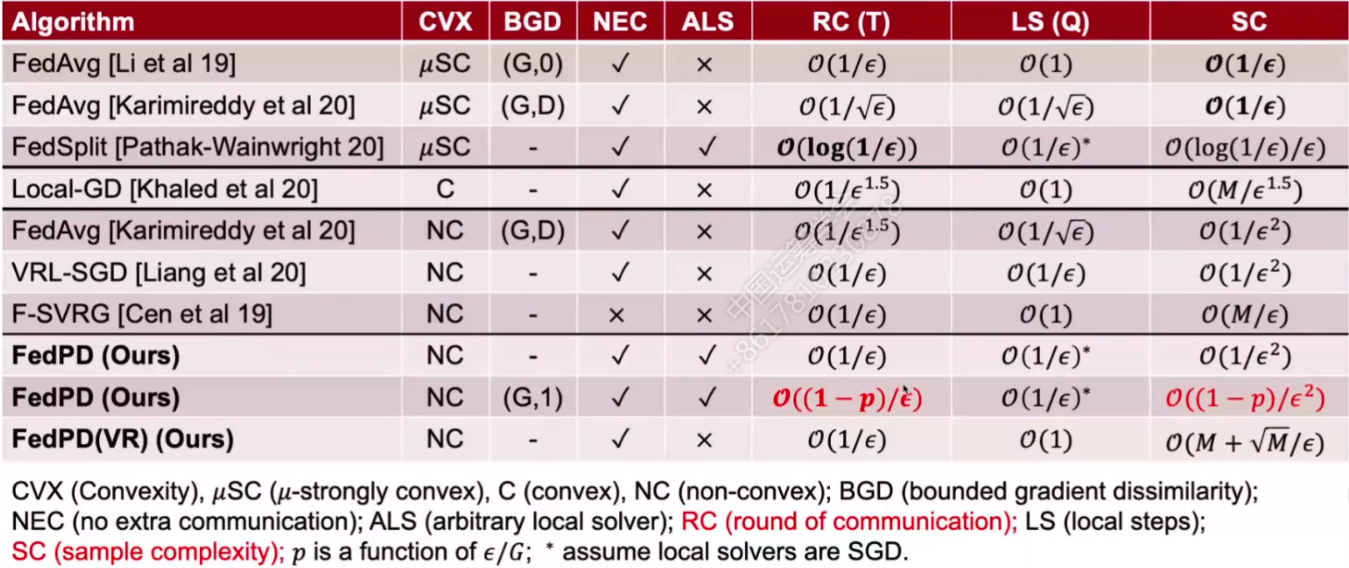
\includegraphics[keepaspectratio,width=0.85\textwidth]{images/mingyi_hong_fedpd.png}
\end{figure}
上图来自洪明毅老师在第六十一期运筹千里纵横论坛所作的报告。

\pause
\vspace{0.4em}

洪明毅老师最近的工作\cite{khanduri2021stem},在进行local update的时候也用了momentum加速,进一步扩展了FedOpt。

\blfootnote{\tiny \cite{khanduri2021stem}\bibentry{khanduri2021stem}}

\end{frame}

%------------------------------------------------

\section{Personalization}

%------------------------------------------------

\begin{frame}
\frametitle{Personalization for FL}

{\bfseries What is model personalization for FL}

\vspace{0.2em}

\noindent --- different models (parameters) for different clients

\pause
\vspace{0.6em}

{\bfseries When does one need personalization?}

\vspace{0.2em}

\noindent --- When data across clients are ``enough'' non-IID and clients do not generally have enough training data, which is more realistic.

\pause
\vspace{0.6em}

{\bfseries Means of personalization:}
\begin{itemize}
    \item Local Fine-tuning.
    \item Model-Agnostic Meta Learning, e.g. \cite{finn2017maml}
    \item Federated Multi-Task Learning (+ regularization / proximal term), e.g. \cite{smith2017mocha}
    \item etc.
\end{itemize}

\end{frame}

%------------------------------------------------

\subsection[MAML]{Model-Agnostic Meta Learning}

%------------------------------------------------
% Page 15

\begin{frame}
\frametitle{Model-Agnostic Meta Learning}

\begin{quote}
    ``The goal of meta-learning is to train a model on a {\bfseries variety of {\color{red} learning tasks}}, such that it can solve new learning tasks using only a small number of training samples.'' \hfill -- \cite{finn2017maml}
\end{quote}

\vspace{0.6em}

i.e. over a distribution of learning tasks $p(\mathcal{T})$, where
$$\mathcal{T} = \{ \mathcal{L}(\{(x_t,a_t)\}), q(x_1), q(x_{t+1}|x_t, a_t), H \}$$
with
\begin{align*}
    & (x_t,a_t): & \text{data points} \\
    & \mathcal{L}: & \text{loss function} \\
    & q(x_1): & \text{initial distribution} \\
    & q(x_{t+1}|x_t, a_t): & \text{transition} \\
    & H: & \text{episode length}
\end{align*}

\end{frame}

%------------------------------------------------
% Page 15

\begin{frame}
\frametitle{Model-Agnostic Meta Learning -- Intuition}

\begin{block}{Intuition of MAML}
Some internal representations are more transferrable than others. MAML should encourage the emergence of such general-purpose representations via searching for model parameters that are sensitive to changes in the task.
\end{block}

\begin{figure}
    \centering
    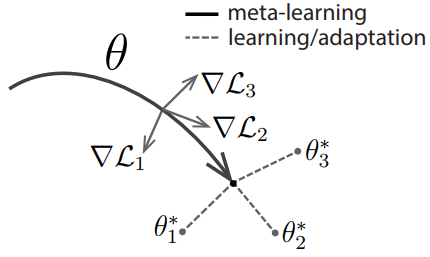
\includegraphics[keepaspectratio,width=.65\textwidth]{images/maml.png}
\end{figure}

\end{frame}

%------------------------------------------------
% Page 15

\begin{frame}
\frametitle{Model-Agnostic Meta Learning -- Formulation}

Mathematically, MAML can be formulated as a (bi-level?) optimization problem
\begin{align*}
    & \text{minimize} \quad \sum\limits_{\mathcal{T}_i\sim p(\mathcal{T})} \mathcal{L}_{\mathcal{T}_i} (f_{\theta_i'}) \\
    & \text{where} \quad \theta_i' = \theta - \alpha \nabla_{\theta} \mathcal{L}_{\mathcal{T}_i}(f_{\theta})
\end{align*}

\begin{figure}
    \centering
    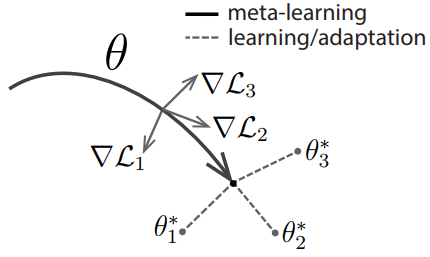
\includegraphics[keepaspectratio,width=.65\textwidth]{images/maml.png}
\end{figure}

\end{frame}

%------------------------------------------------
% Page 15

\begin{frame}
\frametitle{Model-Agnostic Meta Learning -- Algorithm}

\begin{algorithm}[H]
\SetAlgoNoLine
\DontPrintSemicolon
{\bfseries Require:} $p(\mathcal{T})$ distribution over tasks\;
{\bfseries Require:} $\alpha, \beta$ step size hyper-params\;
randomly initialize model params $\theta$\;
\While{not done}{
    Sample batch of tasks $\mathcal{T}_i \sim p(\mathcal{T})$\;
    \For{all $\mathcal{T}_i$}{
        Evaluate $\nabla_{\theta} \mathcal{L}_{\mathcal{T}_i}(f_{\theta})$ w.r.t. $K$ samples\;
        Compute adapted parameters with gradient descent $\theta'_i = \theta - \alpha \nabla_{\theta} \mathcal{L}_{\mathcal{T}_i}(f_{\theta})$\;
    }
    Update \colorbox{pink}{$\theta \leftarrow \theta - \beta \nabla_{\theta} \framebox{$\sum\limits_{\mathcal{T}_i\sim p(\mathcal{T})}$} \mathcal{L}_{\mathcal{T}_i} (f_{\theta_i'})$} \;
}
\caption{MAML\cite{finn2017maml}}
\end{algorithm}

\pause

``Extragradient method''!

\end{frame}

%------------------------------------------------
% Page 15

\begin{frame}
\frametitle{Model-Agnostic Meta Learning -- Applications}

In deep learning, a very commonly used architecture is as follows:
$$\text{input} \to \framebox{CNN (encoder)} ( \to \text{attn}) \to \text{task specific module}$$

tasks can be one or more of
\begin{itemize}
    \item classification (global pooling + linear)
    \item sequence labelling (linear)
    \item segmentation (upsample)
    \item object detection
    \item etc.
\end{itemize}
or many sub-tasks of the above (current main concern for meta-learning).

MAML forces the feature extractor (or called encoder, etc.) to capture general-purpose internal representations (features).

\end{frame}

%------------------------------------------------

\subsection[FMTL]{Federated Multi-Task Learning}

%------------------------------------------------
% Page 15

\begin{frame}
\frametitle{Federated Multi-Task Learning}

\begin{itemize}
    \item pFedMe (bi-level) \cite{t2020pfedme} (and similarly EASGD\cite{zhang2015easgd}):
    \begin{align*}
        & \text{minimize} \quad \sum\limits_{i=1}^N F_i(x), \\
        & \text{where} \quad F_i(x) = \min \left\{ f_i(x_i) + \dfrac{\lambda}{2} \lVert x_i - {\color{red} x}\rVert^2 \right\}
    \end{align*}
    \pgfsetfillopacity{0.4}
    {\footnotesize
    \item FedU \cite{dinh2021fedu}:
    $$\text{minimize} \quad \sum\limits_{i=1}^N f_i(x_i) + \dfrac{\lambda}{2} \sum\limits_{i=1}^N {\color{red} \sum\limits_{j\in\mathcal{N}_i}} \lVert x_i - {\color{red} x_j} \rVert^2$$
    }
    \pgfsetfillopacity{1}
\end{itemize}

\blfootnote{\tiny \cite{t2020pfedme}\bibentry{t2020pfedme}}
\blfootnote{\tiny \cite{zhang2015easgd}\bibentry{zhang2015easgd}}
\blfootnote{\tiny \cite{dinh2021fedu}\bibentry{dinh2021fedu}}

\end{frame}

%------------------------------------------------
% Page 15

\begin{frame}
\frametitle{pFedMe -- Formulation}

pFedMe (Personalized Federated Learning with Moreau Envelopes (or proximity operator)) is formulated as the following bi-level optimization problem in \cite{t2020pfedme}

\begin{align*}
    & \text{minimize} \quad \sum\limits_{i=1}^N F_i(x), \\
    & \text{where} \quad F_i(x) = \min \left\{ f_i(x_i) + \dfrac{\lambda}{2} \lVert x_i - x \rVert^2 \right\}
\end{align*}
which is equivalent to
\begin{align*}
    & \text{minimize} \quad \sum\limits_{i=1}^N \left( f_i(x_i) + \dfrac{\lambda}{2} \lVert x_i - x \rVert^2 \right)
\end{align*}

\blfootnote{\tiny \cite{t2020pfedme}\bibentry{t2020pfedme}}

\end{frame}

%------------------------------------------------
% Page 15

\begin{frame}
\frametitle{pFedMe -- Algorithm}

\begin{algorithm}[H]
\SetAlgoNoLine
\DontPrintSemicolon
{\bfseries Input:} $T,R,S,\lambda,\eta,\beta,x^0$\;
\For{$t = 0,\cdots,T-1$}{
    Server sends $x^t$ to all clients\;
    \For{$i = 1,\cdots,N$}{
        $x_{i,0}^t = x^t$\;
        \For{$r = 0,\cdots, R-1$}{
            Sample a fresh mini-batch $\mathcal{D}_i$, and find an approximate $x_i(x_{i,r}^t)$ to the problem $\text{min} \{ \ell_i(x_i;\mathcal{D}_i) + \frac{\lambda}{2}\lVert x_i-x_{i,r}^t \rVert^2 \}$\;
            Local update $x_{i,r+1}^t = x_{i,r}^t - \eta\lambda(x_{i,r}^t-x_i(x_{i,r}^t))$\;
        }
        Server uniformly samples a subset of clients $\mathcal{S}^t$, each of which sends the local $x_{i,R}^t$ to the server\;
    }
    Sever update $x^{t+1} = (1-\beta)x^t + \beta \sum \frac{x_{i,R}^t}{\# \mathcal{S}^t}$
}
\caption{pFedMe\cite{t2020pfedme}}
\end{algorithm}

\end{frame}

%------------------------------------------------
% Page 15

\begin{frame}
\frametitle{pFedMe -- Algorithm}

\begin{block}{pFedMe observations}
\begin{itemize}
    \item global model $x$ converges (if converges) to the average of local models, which can be inferred from
    $$x^* = \min_{x} \left\{ \sum\limits_{i=1}^N \left( f_i(x_i) + \dfrac{\lambda}{2} \lVert x_i - x \rVert^2 \right) \right\} = \frac{1}{N} \sum\limits_{i=1}^N x_i$$
    \item local updates are not ``totally local'', i.e. the loop $r = 0, \cdots, R$ computes the ``global objective'' $\min\{F_i(x)\}$ locally, to reduce communication.
    \item pFedMe = Method 1 proposed by Caihua Chen, i.e. outer line search of $x$, inner solving $\operatorname{Prox}$
    \item What is Method 2 (randomization?) proposed by Caihua Chen?
\end{itemize}
\end{block}

\end{frame}

%------------------------------------------------

\subsection[Mixture FL]{Mixture Federated Learning}

%------------------------------------------------
% Page 15

\begin{frame}
\frametitle{Mixture FL}

The {\color{red} ``weak'' consensus problem} (originally stated as ``mixture'' FL problem)
$$\text{minimize} \quad \sum\limits_{i=1}^N f_i(x_i) + \dfrac{\lambda}{2} \sum\limits_{i=1}^N \lVert x_i - \overline{x} \rVert^2$$
can be reformulated as constrained optimization problems
\begin{align*}
    & \text{minimize} \quad \sum\limits_{i=1}^N f_i(x_i) + \dfrac{\lambda}{2} \sum\limits_{i=1}^N \lVert x_i - z \rVert^2 \\
    & \text{subject to} \quad Nz - \sum\limits_{i=1}^N x_i = 0
\end{align*}

\end{frame}

%------------------------------------------------
% Page 15

\begin{frame}
\frametitle{Mixture FL}

or equivalently as the following problem,
\begin{align*}
    & \text{minimize} \quad \sum\limits_{i=1}^N f_i(x_i) + \dfrac{\lambda}{2} \sum\limits_{i=1}^N \lVert x_i \rVert^2 -\dfrac{\lambda N}{2} \lVert z \rVert^2 \\
    & \text{subject to} \quad Nz - \sum\limits_{i=1}^N x_i = 0
\end{align*}
which is a nonconvex sharing problem considered in \cite{hong2016convergence} (Eq. (3.2)). Note the difference of between formulations of a sharing problem in \cite{hong2016convergence} (Section 3) and in \cite{boyd2011distributed} (Section 7.3)

\blfootnote{\tiny \cite{hong2016convergence}\bibentry{hong2016convergence}}
\blfootnote{\tiny \cite{boyd2011distributed}\bibentry{boyd2011distributed}}

\end{frame}

%------------------------------------------------
% Page 15

\begin{frame}
\frametitle{Mixture FL}

The algorithm ``Flexible ADMM'' proposed in \cite{hong2016convergence} (Algorithm 4) updates $x_i$ using Gauss-Seidel method, which is non-trivial (or impossible) for parallelization. On the other hand, Jacobi method seems to have no guarantee of convergence.

\blfootnote{\tiny \cite{hong2016convergence}\bibentry{hong2016convergence}}

\end{frame}

%------------------------------------------------
% Page 15

\begin{frame}
\frametitle{Mixture FL}

Under certain assumptions, this problem is a (split?) DC (difference-of-convex) programming problem {\color{red} with linear constraints}.

\begin{align*}
    & \text{minimize} \quad \colorbox{green}{$\sum\limits_{i=1}^N \left( f_i(x_i) + \dfrac{\lambda}{2} \lVert x_i \rVert^2 \right)$} - \lambda \colorbox{pink}{$\dfrac{N}{2} \lVert z \rVert^2$} \\
    & \text{subject to} \quad Nz - \sum\limits_{i=1}^N x_i = 0
\end{align*}

One writes $\widetilde{f}_i (x_i) =  f_i(x_i) + \dfrac{\lambda}{2} \lVert x_i \rVert^2,$ and $r(z) = \frac{N}{2} \lVert z \rVert^2$.

\end{frame}

%------------------------------------------------
% Page 15

\begin{frame}
\frametitle{Mixture FL}

The original unconstrained problem is studied in \cite{hanzely2020federated} using the so-called {\color{red} loopless} local gradient descent (L2GD) method, with the assumptions that
\begin{itemize}
    \item $f_i$ are Lipschitz $L$-smooth
    % $$\lVert \nabla f_i(x) - \nabla f_i(y) \rVert \leqslant L \lVert x-y \rVert$$
    $$f(y) \leqslant f(x) + \langle \nabla f(x), (y-x)\rangle + \dfrac{L}{2} \lVert x-y \rVert^2$$
    \item $f_i$ are $\mu$-strongly convex
    $$f(y) \geqslant f(x) + \langle \nabla f(x), (y-x)\rangle + \dfrac{\mu}{2} \lVert x-y \rVert^2$$
\end{itemize}

{\color{red} Looplessness} is the one of the key contribution of \cite{hanzely2020federated}, in which {\bfseries inner (local) loops are replaced with probabilistic gradient updates}.

\blfootnote{\tiny \cite{hanzely2020federated}\bibentry{hanzely2020federated}}

\end{frame}

%------------------------------------------------
% Page 15

\begin{frame}
\frametitle{Mixture FL}

Rewrite $\sum\limits_{i=1}^N f_i(x_i) + \frac{\lambda}{2} \sum\limits_{i=1}^N \lVert x_i - \overline{x} \rVert^2$ as $f(x) + \psi(x)$ with $x = (x_1,\cdots,x_N)$, the local step of L2GD at a client $i$ is
$$x^{k+1} = x^k - \alpha G(x^k)$$
where
$$
G(x^k) = \begin{cases}
\dfrac{\nabla f(x^k)}{1-p} & \text{ with probability } 1-p \\
\dfrac{\lambda \nabla \psi(x^k)}{p} & \text{ with probability } p 
\end{cases}
$$
Locally, one has
$$x_i^{k+1} = x_i^k - \beta \nabla f_i(x_i^k), \quad x_i^{k+1} = (1-\gamma)x_i^k + \gamma \overline{x}^k$$
with probabilities $1-p$ and $p$ respectively.

\end{frame}

%------------------------------------------------
% Page 15

\begin{frame}
\frametitle{Mixture FL --- ADMM}

\begin{block}{Questions}
\begin{itemize}
    \item[1.] Assumptions on the objective functions can be loosened?
    \item[2.] DCA with linear constraints? (augmented) Lagrangian is
    {\scriptsize
    $$\mathcal{L}_{\rho}(x,z,y) = \sum\limits_{i=1}^N \widetilde{f}_i(x_i) - \lambda r(z) + \langle y, Nz - \sum\limits_{i=1}^N x_i \rangle + \framebox{$\dfrac{\rho}{2} \lVert Nz - \sum\limits_{i=1}^N x_i \rVert^2$} $$
    }
    \item[3.] DCA (or stochastic, accelerated variants) can have better convergence?
    \item[4.] more
\end{itemize}
\end{block}

\end{frame}

%------------------------------------------------
% Page 15

\begin{frame}
\frametitle{Mixture FL --- ADMM}

Because of the existence of the boxed term $\dfrac{\rho}{2} \lVert Nz - \sum\limits_{i=1}^N x_i \rVert^2$, the only choice to fit in the distributed settings is to update using the Jacobi method, as follows:
{\footnotesize
\begin{align*}
    x_i^{k+1} & = \argmin_{x_i} \left\{ \widetilde{f}_i(x_i) - \langle y_i^k, x_i \rangle + \colorbox{pink}{$\displaystyle \frac{\rho}{2} \lVert Nz^k - \sum\limits_{j\neq i}^N x_j^k - x_i \rVert^2$} \right\} \\
    z^{k+1} & = \argmin_{z} \left\{ \langle y^k, Nz \rangle + \frac{\rho}{2} \lVert Nz - \sum\limits_{i=1}^N x_i^{k+1} \rVert^2 - \lambda r(z) \right\} \\
    y^{k+1} & = y^k + \beta (Nz^{k+1} - \sum\limits_{i=1}^N x_i^{k+1})
\end{align*}
}

\end{frame}

%------------------------------------------------
% Page 15

\begin{frame}
\frametitle{Mixture FL --- ADMM}

One can add more intermediate variables and reformulates the DC-like sharing problem as
\begin{align*}
    & \text{minimize} \quad \sum\limits_{i=1}^N \widetilde{f}_i(x_i) - \lambda r(z) \\
    & \text{subject to} \quad x_i' = x_i, \quad i=1,\cdots,N \\
    & \phantom{subject to} \quad Nz = \sum\limits_{i=1}^N x_i'
\end{align*}
Augmented Lagrangian of the above problem is
{\footnotesize
\begin{multline*}
    \sum\limits_{i=1}^N \widetilde{f}_i(x_i) - \lambda r(z) + \sum\limits_{i=1}^N \langle y_i, x_i'-x_i\rangle + \sum\limits_{i=1}^N \dfrac{\rho_i}{2} \lVert x_i'-x_i \rVert^2 \\
    + \langle y, Nz-\sum\limits_{i=1}^N x_i'\rangle + \dfrac{\rho}{2} \left\lVert Nz-\sum\limits_{i=1}^N x_i' \right\rVert^2
\end{multline*}
}

\end{frame}

%------------------------------------------------
% Page 15

\begin{frame}
\frametitle{Mixture FL  --- ADMM}

ADMM iterations of the above problem are
{\footnotesize
\begin{align*}
    x_i^{k+1} & = \argmin_{x_i} \left\{ \widetilde{f}_i(x_i) + \frac{\rho_i}{2} \lVert x_i-(x_i')^k \rVert^2 - \langle y_i^k, x_i \rangle \right\} \\
    (x_i')^{k+1} & = \argmin_{x_i'} \left\{ \langle y_i^k-y^k, x_i' \rangle + \frac{\rho_i}{2} \lVert x_i^{k+1}-x_i' \rVert^2 \right. \\
    & \hspace{7em} + \colorbox{pink}{$\displaystyle \frac{\rho}{2} \lVert Nz^k-\sum\limits_{j\neq i}^N (x_j')^{k} - x_i' \rVert^2$} \} \\
    z^{k+1} & = \argmin_{z} \left\{ \langle y^k, Nz \rangle + \frac{\rho}{2} \lVert Nz - \sum\limits_{i=1}^N (x_i')^{k+1} \rVert^2 - \lambda r(z) \right\} \\
    y_i^{k+1} & = y_i^k + \beta ((x_i')^{k+1} - x^{k+1}) \\
    y^{k+1} & = y^k + \beta (Nz^{k+1} - \sum\limits_{i=1}^N (x_i')^{k+1})
\end{align*}
}

\end{frame}

%------------------------------------------------
% Page 15

\begin{frame}
\frametitle{Huawei Noah FL Workshop}

\begin{figure}
    \centering
    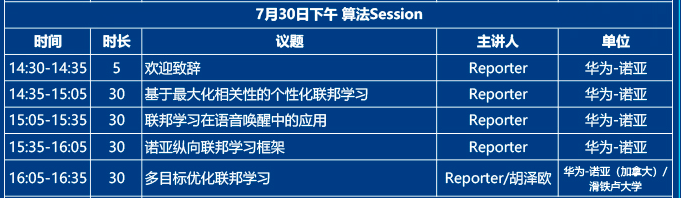
\includegraphics[keepaspectratio,width=\textwidth]{images/huawei_noah_fl_workshop.png}
\end{figure}

\end{frame}

%------------------------------------------------

\section{Compression}

%------------------------------------------------
% Page 15

\begin{frame}
\frametitle{Compression in Federated Learning}

As is discussed previously (e.g. in the study of ``GADMM'' to ``CQ-GGADMM''), one of the main bottleneck {\color{red} communication cost} can be reduced using
\begin{itemize}
    \item compression
    \item {\pgfsetfillopacity{0.3}lazy aggregation (censoring)}
    \item {\pgfsetfillopacity{0.3}etc.}
\end{itemize}

\pause
\vspace{0.6em}

\pgfsetfillopacity{1}
The technique of compression mainly consists of
\begin{itemize}
    \item (randomized) quantization
    \item sparsification
\end{itemize}
or their combination.

\end{frame}

%------------------------------------------------

\subsection{Naive Compression Methods}

%------------------------------------------------
% Page 2

\begin{frame}
\frametitle{Deterministic Compression}

compression can be naively done via fixed reduction of precision (fixed bit of quantization) of parameters and/or gradients, e.g. {\color{red} half precision} (\texttt{float32} $\to$ \texttt{float16}) or {\color{red} mixed precision}.

\vspace{0.6em}

This is the common practice for acceleration of ordinary (non-distributed) model training process. e.g. the \href{https://pytorch.org/blog/accelerating-training-on-nvidia-gpus-with-pytorch-automatic-mixed-precision/}{\beamergotobutton{PyTorch Post}} on mixed precision training.

\end{frame}

%------------------------------------------------
% Page 3

\begin{frame}
\frametitle{TernGrad}

One extreme case of compression is to take the {\color{red}sign} of each coordinate of the stochastic gradient vector, which makes it binary (1-bit, $\pm 1$) or ternary ($\{-1, 0, +1\}$).

\vspace{0.4em}

\begin{columns}
\begin{column}{0.44\textwidth}
\begin{figure}
    \centering
    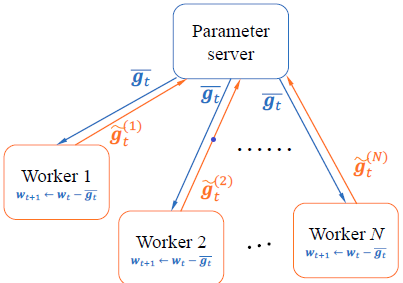
\includegraphics[width=1\textwidth,keepaspectratio]{images/terngrad.png}
\end{figure}
\end{column}
\begin{column}{0.52\textwidth}
$\widetilde{g}_t^{(i)}$ is the {\color{red}ternarized} gradient
$$g_t^{(i)} = \lVert g_t^{(i)} \rVert_{\infty} \cdot \operatorname{sign}(g_t^{(i)}) \odot \framebox{\color{red} $b_t$}$$
where $b_t$ is a random binary vector satisfying some Bernoulli distribution $Be(\lvert g_{t,k}^{(i)} \rvert / s_t)$
\end{column}
\end{columns}

\vspace{0.4em}

Similar algorithms include 1-bit SGD \cite{seide2014_1bitsgd}, signSGD \cite{bernstein2018signsgd}

\blfootnote{
\tiny\cite{seide2014_1bitsgd} \bibentry{seide2014_1bitsgd}
}
\blfootnote{
\tiny\cite{bernstein2018signsgd} \bibentry{bernstein2018signsgd}
}

\end{frame}

%------------------------------------------------
% Page 3

\begin{frame}
\frametitle{QSGD}

More generally, in QSGD \cite{alistarh2017qsgd}, randomized quantization (called ``low-precision quantizer'' in \cite{khirirat2018dcgd}) is performed on gradients $v$ via
$$Q_s(v) = \lVert v \rVert_2 \cdot \operatorname{sign}(v) \odot \framebox{\color{red}$\xi(v,s)$},$$
where the $i$-th element in vector $\xi(v,s)$ is defined by
\begin{equation*}
    \xi_i(v,s) = \begin{cases}
    (\ell+1)/s, & \text{with prob. } (|v_i|/\lVert v \rVert_2) s - \ell \\
    \ell/s, & \text{otherwise}
    \end{cases}
\end{equation*}
$s$ controls the number of quantization levels, and $\ell$ ({\color{red} should be $\ell_i$?}) be s.t. $|v_i|/\lVert v \rVert_2 \in [\ell/s, (\ell+1)/s]$.

\blfootnote{
\tiny\cite{alistarh2017qsgd} \bibentry{alistarh2017qsgd}
}
\blfootnote{
\tiny\cite{khirirat2018dcgd} \bibentry{khirirat2018dcgd}
}

\end{frame}

%------------------------------------------------
% Page 3

\begin{frame}
\frametitle{DCGD}

DCGD \cite{khirirat2018dcgd} generalized such operators $Q_s$ into an abstract concept

\begin{Def}[Unbiased Random Quantizer (URQ)]
A mapping $Q:\mathbb{R}^d \to \mathbb{R}^d$ is called an unbiased random quantizer if $\forall v \in \mathbb{R}^d$,
\begin{itemize}
    \item $\operatorname{supp}(Q(v)) \subseteq \operatorname{supp}(v)$
    \item $\expectation [Q(v)] = v$
    \item $\expectation [\lVert Q(v) \rVert_2^2] \leqslant \alpha \lVert v \rVert_2^2$ for some finite positive $\alpha$
\end{itemize}
\end{Def}

And perhaps with more useful properties like
\begin{itemize}
    \item sparsity: $\expectation [\lVert Q(v) \rVert_0] \leqslant$ const
    \item sign preserving: $Q(v)_i \cdot v_i \geqslant 0$
\end{itemize}

\blfootnote{
\tiny\cite{khirirat2018dcgd} \bibentry{khirirat2018dcgd}
}

\end{frame}

%------------------------------------------------
% Page 3

\begin{frame}
\frametitle{Examples of URQs}

Despite the ternary quantizer and low-precision quantizer, one has \cite{lizhize2020adiana}

\only<1>{
\begin{block}{Random-$k$ sparsification}
$$\mathcal{C}(v) = \dfrac{d}{k} (v \odot \xi_k)$$
where $\xi_k \in \{0, 1\}^d$ is a uniformly random binary vector with $k$ nonzero entries, $v \in \mathbb{R}^d$.
\end{block}
}

\only<2>{
\begin{block}{$(p,s)$-quantization}
$$\mathcal{C}_{p,s}(v) = \operatorname{sign}(v)\cdot \lVert v \rVert_p \cdot \dfrac{1}{s} \xi(v,s)$$
where $\xi(v,s)$ is a random vector with i-th element
\begin{equation*}
\xi_i(v,s) = \begin{cases}
\ell_i+1, & \text{with prob. } (|v_i|/\lVert v \rVert_2) s - \ell_i \\
\ell_i, & \text{otherwise}
\end{cases}
\end{equation*}
and $\ell_i$ be s.t. $|v_i|/\lVert v \rVert_2 \in [\ell_i/s, (\ell_i+1)/s]$
\end{block}
}

\blfootnote{
\tiny\cite{lizhize2020adiana} \bibentry{lizhize2020adiana}
}

\end{frame}

%------------------------------------------------
% Page 3

\begin{frame}
\frametitle{Implementations of Quantizers}

One can refer to \href{https://github.com/burlachenkok/marina}{\beamergotobutton{https://github.com/burlachenkok/marina}} for code and examples of various compressors, e.g. in files
\begin{itemize}
    \item \href{https://github.com/burlachenkok/marina/blob/main/linear_model_with_non_convex_loss/compressors.py}{\beamergotobutton{linear\_model\_with\_non\_convex\_loss/compressors.py}}
    \item \href{https://github.com/burlachenkok/marina/blob/main/neural_nets_experiments/compressors.py}{\beamergotobutton{neural\_nets\_experiments/compressors.py}}
\end{itemize}

\vspace{0.8em}

or \href{https://github.com/wenh06/fl_seminar/blob/master/code/compressors_test.ipynb}{\beamergotobutton{this simple jupyter notebook}}

\end{frame}

%------------------------------------------------

\subsection{Recent Development}

%------------------------------------------------
% Page 3

\begin{frame}
\frametitle{(A)DIANA}

The main contribution of (A)DIANA \cite{lizhize2020adiana,mishchenko2019diana} is that, instead of quantizing the gradients, the {\color{red} difference of gradient updates}, i.e. instead of
$$\widetilde{g}^{(i)}_t = Q(g^{(i)}_t) = Q(\nabla f_i(x_t))$$
one performs
\begin{equation*}
    \begin{cases}
    \widetilde{g}^{(i)}_t = h^{(i)}_t + Q(\colorbox{pink}{$\nabla f_i(x_t) - h^{(i)}_t$}) \\
    \colorbox{pink}{$h^{(i)}_{t+1} = h^{(i)}_t + \alpha Q(\nabla f_i(x_t) - h^{(i)}_t)$}
    \end{cases}
\end{equation*}

$h^{(i)}$ are ``memory'' maintained locally, whose average is maintained in the central server.

\blfootnote{
\tiny\cite{lizhize2020adiana} \bibentry{lizhize2020adiana}
}
\blfootnote{
\tiny\cite{mishchenko2019diana} \bibentry{mishchenko2019diana}
}

\end{frame}

%------------------------------------------------
% Page 3

\begin{frame}
\frametitle{(A)DIANA}

Another key point (feature) of (A)DIANA is the combination with acceleration (and variance reduction):

\only<1>{
\begin{figure}
    \centering
    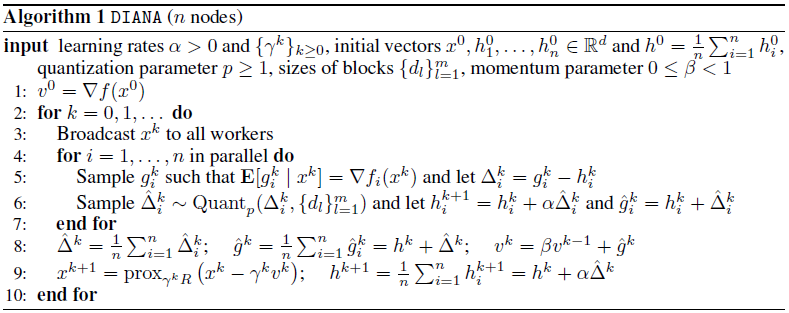
\includegraphics[width=0.9\textwidth,keepaspectratio]{images/diana.png}
\end{figure}

{\footnotesize Note the ``Quant'' operator is a so-called ``block-quantizer'' or ``bucket-quantizer''\cite{alistarh2017qsgd} {\tiny \bibentry{alistarh2017qsgd}}
}}
\only<2>{
\begin{figure}
    \centering
    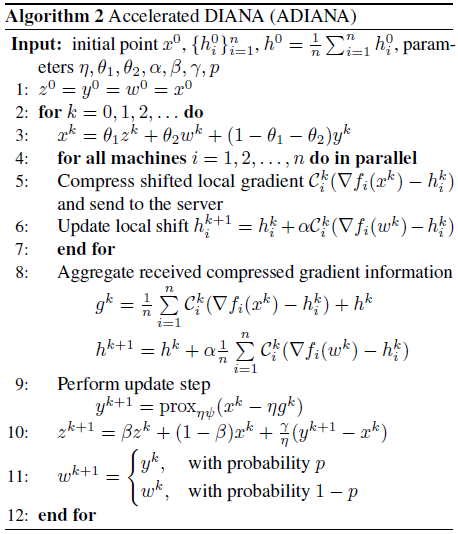
\includegraphics[width=0.54\textwidth,keepaspectratio]{images/adiana.png}
\end{figure}
}

\end{frame}

%------------------------------------------------
% Page 3

\begin{frame}
\frametitle{MARINA}

MARINA \cite{gorbunov2021marina} replaced the unbiased compressor by a {\color{red}biased} one, via replacing
\begin{equation*}
\begin{cases}
\widetilde{g}^{(i)}_t = h^{(i)}_t + Q(\nabla f_i(x_t) - h^{(i)}_t) \\
h^{(i)}_{t+1} = h^{(i)}_t + \alpha Q(\nabla f_i(x_t) - h^{(i)}_t)
\end{cases}
\end{equation*}
by
\begin{equation*}
\widetilde{g}^{(i)}_t = 
\begin{cases}
\nabla f_i(x_t), & \text{with prob. } p \\
\widetilde{g}^{(i)}_{t-1} + Q(\nabla f_i(x_t) - \nabla f_i(x_{t-1})), & \text{with prob. } 1-p
\end{cases}
\end{equation*}
for some small $p$.

\uncover<2->{
As claimed by the authors, their intuition come from the rare (?) phenomenon in stochastic optimization that
\begin{quote}
`` the bias of the stochastic gradient helps to achieve better complexity''
\end{quote}
}

\blfootnote{
\tiny\cite{gorbunov2021marina} \bibentry{gorbunov2021marina}
}

\end{frame}

%------------------------------------------------
% Page 3

\begin{frame}
\frametitle{MARINA}

The basic MARINA algorithm is as follows:

\begin{figure}
    \centering
    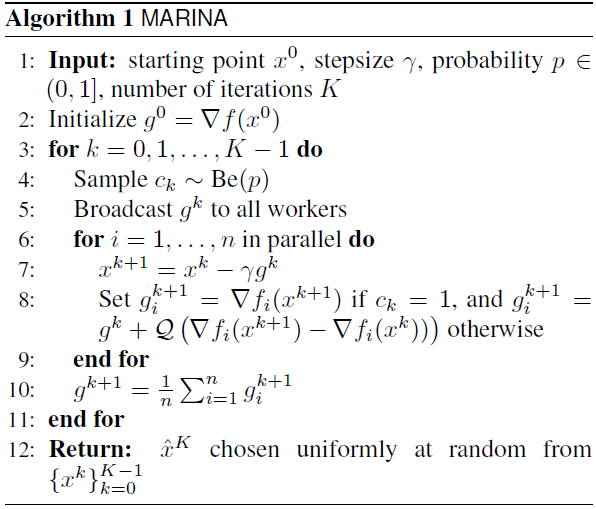
\includegraphics[width=0.7\textwidth,keepaspectratio]{images/marina.png}
\end{figure}

\end{frame}

%------------------------------------------------
% Page 15

\begin{frame}[allowframebreaks]
\frametitle{References}

{\footnotesize
\bibliographystyle{ieeetr}
\bibliography{references}
}

\end{frame}

%------------------------------------------------

\begin{frame}

{\Huge{\centerline{\bfseries The End}}}

\vspace{0.5em}

{\Huge{\centerline{\phantom{a}\bfseries 谢谢!}}}

\vfill

\noindent 以上内容可以在\href{https://github.com/wenh06/fl_seminar}{\beamergotobutton{https://github.com/wenh06/fl\_seminar}}找到。

\end{frame}

%------------------------------------------------

\end{document}
